%%% Local Variables:
%%% mode: latex
%%% TeX-master: t
%%% End:

\documentclass[bachelor,nofonts]{thuthesis}
%\documentclass[master]{thuthesis}
%\documentclass[doctor]{thuthesis}
% \documentclass[%
%   bachelor|master|doctor|postdoctor, % mandatory option
%   winfonts|nofonts|adobefonts, % mandatory only for bachelor and Linuxer
%   secret,
%   openany|openright,
%   arialtoc,arialtitle]{thuthesis}
% 当使用 XeLaTeX 编译时,本科生、Linux 用户需要加上 nofonts 选项;
% 当使用 PDFLaTeX 编译时,adobefonts 选项等效于 winfonts 选项(缺省选项)。

% 所有其它可能用到的包都统一放到这里了,可以根据自己的实际添加或者删除。
\usepackage{thutils}
\usepackage{tikz}
\usepackage{pgfplots}
\usepackage{algorithm}
\usepackage{algorithmicx}
\usepackage{algpseudocode}
\floatname{algorithm}{算法}
\renewcommand{\algorithmicrequire}{\textbf{输入:}}
\renewcommand{\algorithmicensure}{\textbf{输出:}}

% 你可以在这里修改配置文件中的定义,导言区可以使用中文。
% \def\myname{薛瑞尼}

\begin{document}

% 定义所有的eps文件在 figures 子目录下
\graphicspath{{figures/}}


%%% 封面部分
\frontmatter

%%% Local Variables:
%%% mode: latex
%%% TeX-master: t
%%% End:
\secretlevel{绝密} \secretyear{2015}

\ctitle{基于 Spark 的分布式近似近邻查询系统}
% 根据自己的情况选,不用这样复杂
\makeatletter
\ifthu@bachelor\relax\else
  \ifthu@doctor
    \cdegree{工学博士}
  \else
    \ifthu@master
      \cdegree{工学硕士}
    \fi
  \fi
\fi
\makeatother


\cdepartment[软件]{软件学院}
\cmajor{计算机软件}
\cauthor{文庆福}
\csupervisor{王建民教授}
% 如果没有副指导老师或者联合指导老师,把下面两行相应的删除即可。
%\cassosupervisor{陈文光教授}
%\ccosupervisor{某某某教授}
% 日期自动生成,如果你要自己写就改这个cdate
%\cdate{\CJKdigits{\the\year}年\CJKnumber{\the\month}月}

% 博士后部分
% \cfirstdiscipline{计算机科学与技术}
% \cseconddiscipline{系统结构}
% \postdoctordate{2009年7月——2011年7月}

% 这块比较复杂,需要分情况讨论:
% 1. 学术型硕士
%    \edegree:必须为Master of Arts或Master of Science(注意大小写)
%              “哲学、文学、历史学、法学、教育学、艺术学门类,公共管理学科
%               填写Master of Arts,其它填写Master of Science”
%    \emajor:“获得一级学科授权的学科填写一级学科名称,其它填写二级学科名称”
% 2. 专业型硕士
%    \edegree:“填写专业学位英文名称全称”
%    \emajor:“工程硕士填写工程领域,其它专业学位不填写此项”
% 3. 学术型博士
%    \edegree:Doctor of Philosophy(注意大小写)
%    \emajor:“获得一级学科授权的学科填写一级学科名称,其它填写二级学科名称”
% 4. 专业型博士
%    \edegree:“填写专业学位英文名称全称”
%    \emajor:不填写此项


% 这个日期也会自动生成,你要改么?
% \edate{December, 2005}

% 定义中英文摘要和关键字
\begin{cabstract}
  近似近邻查询是处理非结构化数据的一项基本而重要的技术,在模式识别、数据挖掘等前沿研究领域有着广泛的应用。随着数据指数式的增长,如何从大规模高维数据中进行尽
  可能快速、精确地查询成为备受关注的问题。

  本文中,我们通过对比研究了基于树结构的索引方法和基于哈希的索引方法,并介绍了其中具有代表性的几种方法。本文采用向量量化的哈希方法,在 Spark 平台上建立了一套近似近邻
  查询系统,不仅可以降低存储代价,而且在保证高检索准确率的情况下加速查询效率。最终介绍了在三个数据集上进行的实验,验证系统的正确性和可用性。
\end{cabstract}

\ckeywords{近似近邻查询, Spark, 乘积量化, 索引}

\begin{eabstract}
   Approximate nearest neighbor search (ANNS) is a basic and important technique
   in processing unstructured data, which is widely used in frontier research fields,
   such as Pattern Recognition and Data Mining. With exponential growth of data, much
   attention has been paid to the question that how to search in large-scale
   high-dimensional data as fast and accurately as we can.

   In this paper, we study tree-based indexing method and hash-based indexing
   method comparatively, and introduce several representative method of them. We build
   an ANNS system on Spark using hashing method based on vector quantization, which can
   not only reduce storage costs but also improve query efficiency with high accuracy of retrieval. Finally, we introduce
   experiments that are performed on three dataset to validate correctness and practicability
   of the system.
\end{eabstract}

\ekeywords{Approximate Nearest Neighbor Search, Spark, Product Quantization, Indexing}

% 设置 PDF 文档的作者、主题等属性
\makeatletter
\thu@setup@pdfinfo
\makeatother
\makecover

% 目录
\tableofcontents

% 符号对照表
\begin{denotation}

\item[ANNS] 近似近邻查询 (Approximate Nearest Neighbor Search)
\item[PQ] 乘积量化 (Product Quantization)
\item[SDC] 对称距离度量 (Symmetric Distance Computation)
\item[ADC] 非对称距离度量 (Asymmetric Distance Computation)
\item[ITQ] 迭代量化 (Iterative Quantization)
\item[SVD] 奇异值分解 (Sigular Value Decomposition)
\item[API] 应用程序编程接口
\item[RDD] 弹性分布式数据集 (Resilient Distributed Datasets)
\item[$\lVert\cdot\rVert_2$] L$_2$ 范数
\item[$\lVert\cdot\rVert_F$] Frobenius 范数
\item[$h$] 子空间中聚类中心数量
\item[$m$] 子空间个数
\end{denotation}



%%% 正文部分
\mainmatter

%%% Local Variables:
%%% mode: latex
%%% TeX-master: t
%%% End:

\chapter{引言}
\label{cha:introdction}

\section{研究背景}
在今天这个数据爆炸的时代,文本、图像、视频以及音频等多媒体数据呈现出指数级的增长。如何快速、准确地从这个海量的互联网数据库中获取我们想要的信息,是我们不得不面对的一个问题。Google\footnote{https://www.google.com}、Bing\footnote{http://cn.bing.com}、Baidu\footnote{https://www.baidu.com} 等提供的文本、图像等搜索引擎服务为我们获取信息带来了极大的便利。而在这些搜索引擎背后的都需要用到的一项技术——\textbf{近似近邻查询}(Approximate Nearest Neighbor Search)。在大规模数据的应用场景下,精确的近似查询需要耗费时间太长,不具有实际应用价值。近似近邻查询可以大幅度缩短查询时间,同时保证查询结果与精确查询结果近似,因此更具有实用性。除了信息检索以外,近似近邻查询技术被广泛应用于计算机视觉、机器学习、数据挖掘、模式识别等领域。

在不考虑时间效率的情况下,近似近邻查询问题可以直接通过一种暴力搜索的方式来解决。比如,我们可以直接计算查询数据$q$与数据集合$S$ 中每一条数据的距离,最终根据距离大小,选取出距离最近的前$n$个数据。但在现实中,由于数据集合$S$的规模非常,这种朴素的方法单词查询的计算时间太长而无法采用。但是,如果从规模比较大的数据集合$S$上删选出一个非常小待选集合$S'$,之后再在集合$S'$上进行朴素的暴力搜索选取出前$n$个近邻数据,这时的暴力搜索的时间效率是可以接受的,整个查询过程的时间效率和准确率就取决于删除出待选集合$S'$的过程。待选集合$S'$大小与查询准确率有着密切关系,一般来说,集合$S'$越大,查询准确率越高,但是最终的暴力搜索阶段的时间会变长;集合$S'$越小,则查询效率越低,暴力搜索阶段的时间越短。因此,如何选择一个大小合适、相关性高的待选集合$S'$就成了近似近邻查询问题的关键。

近年来,近似近邻查询问题一直都是研究热点问题之一。目前,这一技术主要面临一下两大挑战:
\begin{enumerate}
\item 海量

随着互联网上的数据越来越多,需要存储的数据量也越来越大。然而,传统的索引结构一般都是基于小规模数据而设计的单机结构。大规模的数据一般无法做到单机存储,更不用说加载到内存当中索引了。这些数据往往存储于分布式系统当中,同时也需要一种分布式的索引结构来支持查询。海量的数据不仅给存储带来了压力,同时也给实时查询带来了巨大挑战。
\item 维度灾难

在多媒体数据处理过程时,往往都会针对多媒体数据提取特征进行处理。为了更好地刻画数据,一般来说,特征数据的维度越高,刻画的准确性也越高。例如,在图像数据处理过程中,我们常常可能用到的 SIFT、SURF 特征都是 128 维的,GIST 特征有 960 维,而 BOVW(Bag of Visual Words)的维度更是高达成千上万维。如此高维度的数据,仅计算两个向量之间距离的时间消耗就比较长,更不必说在大规模数据上进行查询了。
\end{enumerate}

Spark 是一个基于 MapReduce 的通用的大数据并行计算框架,最初由 UC Berkeley AMP Lab 开发。Spark 的架构是在 Hadoop 基础上的改良,继承了 MapReduce 的优点,它与 Hadoop 最大不同之处就是内存计算,Hadoop 将计算过程的中间数据存储在磁盘上,而 Spark 一般是用内存来存储数据,所有数据操作都在内存中完成。

\section{主要研究内容}
本文的主要的关注点是在高维空间中的近似近邻查询问题,通过研究对比现有的几种最新近似近邻查询方法,了解几种不同方法的优缺点。在 Spark 框架下实现了一种基于向量量化(Vector Quantization)的近似近邻查询方法。最终,通过实验来验证算法的准确性以及测试算法时间效率。

\section{论文组织结构}

%%% Local Variables:
%%% mode: latex
%%% TeX-master: t
%%% End:

\chapter{索引结构综述}
\label{cha:related-work}
前文已经提到,近邻查询问题最关键的就是如何选取出一个待选集合$S'$。为了高效地删选出待选集合,我们通常会先把原始的数据索引起来。依据
索引结构的不同,近邻查询的方法可以分为基于树结构的索引和基于哈希的索引。
\section{基于树结构的索引}
\subsection{KD-树}
\subsection{K-Means树}
\section{基于哈希的索引}
基于哈希的索引方法是将高维的数据压缩成二进制编码的形式来进行近似近邻查询,这类方法在图像、文本、视频等多媒体检索上取得不错的效果。
根据哈希函数形式的不同,我们可以简单地将哈希索引分为两类——汉明嵌入和向量量化。
\subsection{汉明嵌入}
汉明嵌入就是要寻找一个映射,对于任意的对象$x \in S$都能映射到二进制串$b(x) \in {0,1}^d$。那么,任意两个对象之间的相似度就可以通过
其对应二进制串之间的汉明距离来近似计算:
\begin{equation}
sim(x, y)\thickapprox 1 - \frac{2\delta_{Ham}(b(x),b(y))}{d}
\end{equation}
\subsection{向量量化}
基于向量量化的哈希索引是对原始向量空间进行量化压缩,原始向量$\mathbf{x} \in \mathbb{R}^D$ 通过量化函数 $q$ 被映射到 $q(\mathbf{x}) \in \mathcal{C} = \{\mathbf{c}_i\}$,其中 $i$ 是下标,$\mathbf{c}_i$ 可以称作为码字,而$\mathcal{C}$则被称为码本。 这种映射可以形式化定义成:$\forall \mathbf{x} \in \mathbb{R}^D$,$\exists \mathbf{c}_i \in \mathcal{C} $,$q(\mathbf{x})=\mathbf{c}_i$。整个量化过程中的量化误差 $E$ 就可以定义为:
\begin{equation}
E = \frac{1}{n}\sum_{\mathbf{x}}\lVert \mathbf{x} - q(\mathbf{x}) \rVert ^2
\end{equation}

其中$\lVert \cdot \rVert$ 表示欧氏距离,而 $n$ 是数据的总量。对于给定的原始数据集合 $S$,我们的目标是找到一个码本 $\mathcal{C}$ 以及对应量化函数 $q(\mathbf{x})$ 使得量化误差 $E$ 最小。在最小化量化误差过程中,不同的限制条件就对应了不同的量化方法。
\subsection{K-Means}
假设有一个包含 $n$ 个 $p$ 维 数据点的集合,$\mathcal{D}\{\mathbf{x}_j\}_{j=1}^n$ , k-means 算法会将这 $n$ 个数据点聚成 $k$ 类,同时用聚类中心来代表每一个聚类的数据。假如矩阵$C \in \mathbb{R}^{p\times k}$的列向量由 $k$ 个聚类构成,每一列都是一个聚类中心,$C=[\mathbf{c}_1,\mathbf{c}_2,\cdots, \mathbf{c}_k]$。k-means 量化的目标函数如下:
\begin{eqnarray}
\mathit{l}_\mathrm{k-means} &=&\sum_{\mathbf{x}\in\mathcal{D}}\min_{i}\lVert \mathbf{x} - \mathbf{c}_i \rVert _2^2 \\
                   &=&\sum_{\mathbf{x}\in\mathcal{D}}\min_{\mathbf{b}\in\mathcal{H}_{1/k}}\lVert \mathbf{x} - C\mathbf{b} \rVert _2^2
\end{eqnarray}

其中$\mathcal{H}_{1/k} = \{\mathbf{b}|\mathbf{b}\in\{0,1\}^k$且$\lVert\mathbf{b}\rVert=1\}$,$\mathbf{b}$ 是一个 1 对 $k$ 编码的二进制向量(包含 1 个 1 ,$k$-1 个 0)。

k-means 量化模型浅显易懂,使用最朴素的近邻查询方法就可以将数据点映射到聚类中心。这种映射过程将每一个原始数据压缩到了 $\log_2k$ 比特的数据,所需要消耗的存储空间随着 $k$ 的线性增长。
\subsection{ITQ}
ITQ(Iterative Quantization)\cite{YunchaoGong:2011:IQP:2191740.2191779}的量化方法是在 2011 年的 CVPR 会议上提出,这一方法较之前的哈希方法在准确率上有了显著提升。

ITQ 方法首先是对原始数据集空间进行 PCA 降维,将原始的 $\mathbb{R}^{n\times d}$ 空间降维成 $\mathbb{R}^{n\times c}$ 空间。此时,再
考虑将降维后的数据集进行二进制编码。从降维后的空间中取出$\mathbf{v}\in \mathbb{R}^{c}$,其对应的编码 sgn($\mathbf{v}$) 可以看做事超立方体$\{-1,1\}^c$
中的顶点。此时,欲使整体的量化误差最小,就是要使原始数据与编码后的数据的欧氏距离最小,$\min{\lVert \mathrm{sgn}(\mathbf{v})-\mathbf{v}\rVert ^2}$。
对于编码前的原始数据集我们用 $X \in \mathbb{R}^{n\times d}$ 来表示,经过 PCA 降维后用 $V \in \mathbb{R}^{n\times c}$ 表示,编码后的数据集用 $B \in \{-1,1\}^{n\times c}$ 来表示。
整体量化误差:
\begin{equation}
Q(B, R) = \lVert B - VR \rVert_F ^2
\end{equation}

其中$\lVert \cdot \rVert_F$ 是 Frobenius 范式,而 $R$ 是正交矩阵,作用是对 $V$ 进行旋转对齐。为何要引入这个旋转矩阵 $R$ 呢?从下图(\ref{fig:itq})可以看出,左侧是 PCA 降维后的数据集 $V$,中间是随机旋转后的数据集,右侧是最优化旋转后的数据集 $VR$。右乘一个旋转矩阵 $R$,让待编码的数据绕数据中心进行旋转到合适状态,每个数据点就可以用距离其最近的数据顶点来表示。下图中可以用 $(-1, -1), (-1, 1), (1, 1), (1, -1) $ 这是四个点来表示。此时,所有的数据点到超立方的顶点的距离和最小,也就是量化误差最小。
\begin{figure}[H]
  \centering
  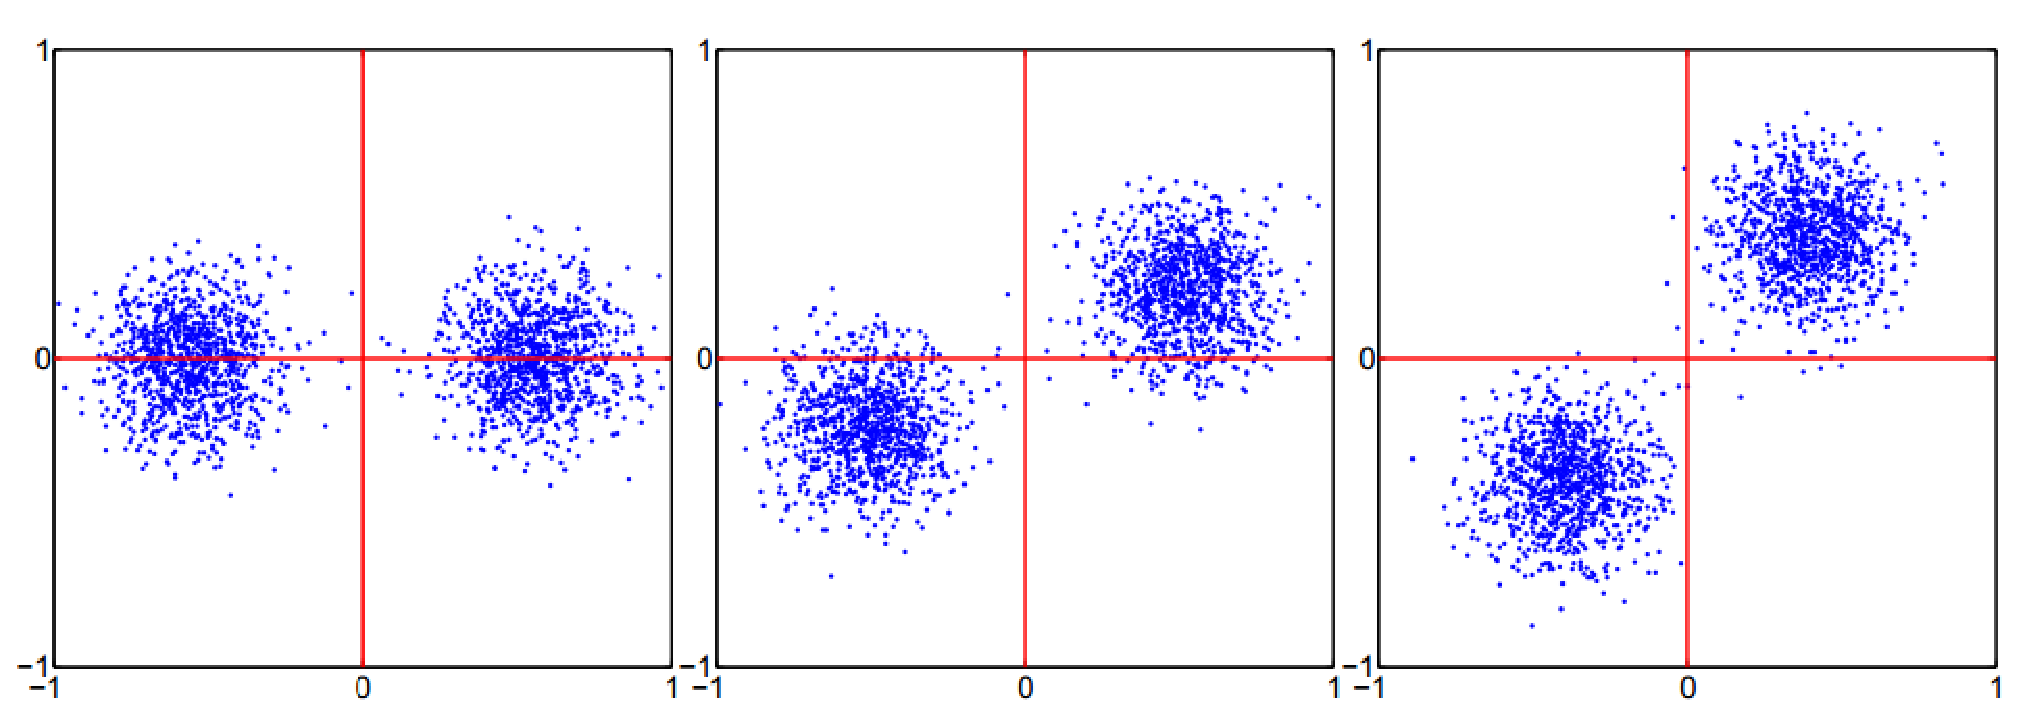
\includegraphics[width=1.0\linewidth]{itq}
  \caption{ITQ 旋转过程}
  \label{fig:itq}
  \footnotesize 注:图像来源\cite{YunchaoGong:2011:IQP:2191740.2191779}
\end{figure}
这样,整个问题的目标函数就变成了$\min \lVert B - VR \rVert_F ^2$。这个公式中有两个未知量,编码后的矩阵 $B$ 和 旋转矩阵 $R$。所以,这个问题的求解要考虑采用交替迭代的方法。先对一个随机生成的矩阵进行 SVD 分解得到一个正交矩阵作为 $R$ 的初始值,此时 $R$ 已知,就可以用$ B= \mathrm{sgn}(VR)$ 来求解 $B$;当 $B$ 已知后,可以对 $B^TV$ 进行 SVD 分解求解 $R$。既然 $R$ 求出,又可以重新一次迭代,固定 $R$ 求 $B$,如此交替迭代就可以求解出该问题。
\subsection{Cartesian K-Means}



%%% Local Variables:
%%% mode: latex
%%% TeX-master: t
%%% End:

\chapter{基于 Spark 的分布式近似近邻查询系统}
\label{cha:ANNS_based_on_Spark}
\section{Spark 的弹性分布式数据集与分布式机器学习库}
Spark 是一个基于 MapReduce 的通用的大数据并行计算框架,最初由 UC Berkeley AMP Lab 开发。Spark 的架构是在 Hadoop 基础上的改良,继承了 MapReduce 的优点,它与 Hadoop 最大不同之处就是内存计算,Hadoop 将计算过程的中间数据存储在磁盘上,而 Spark 一般是用内存来存储数据,从而提高计算效率。
\begin{figure}[H]
  \centering
  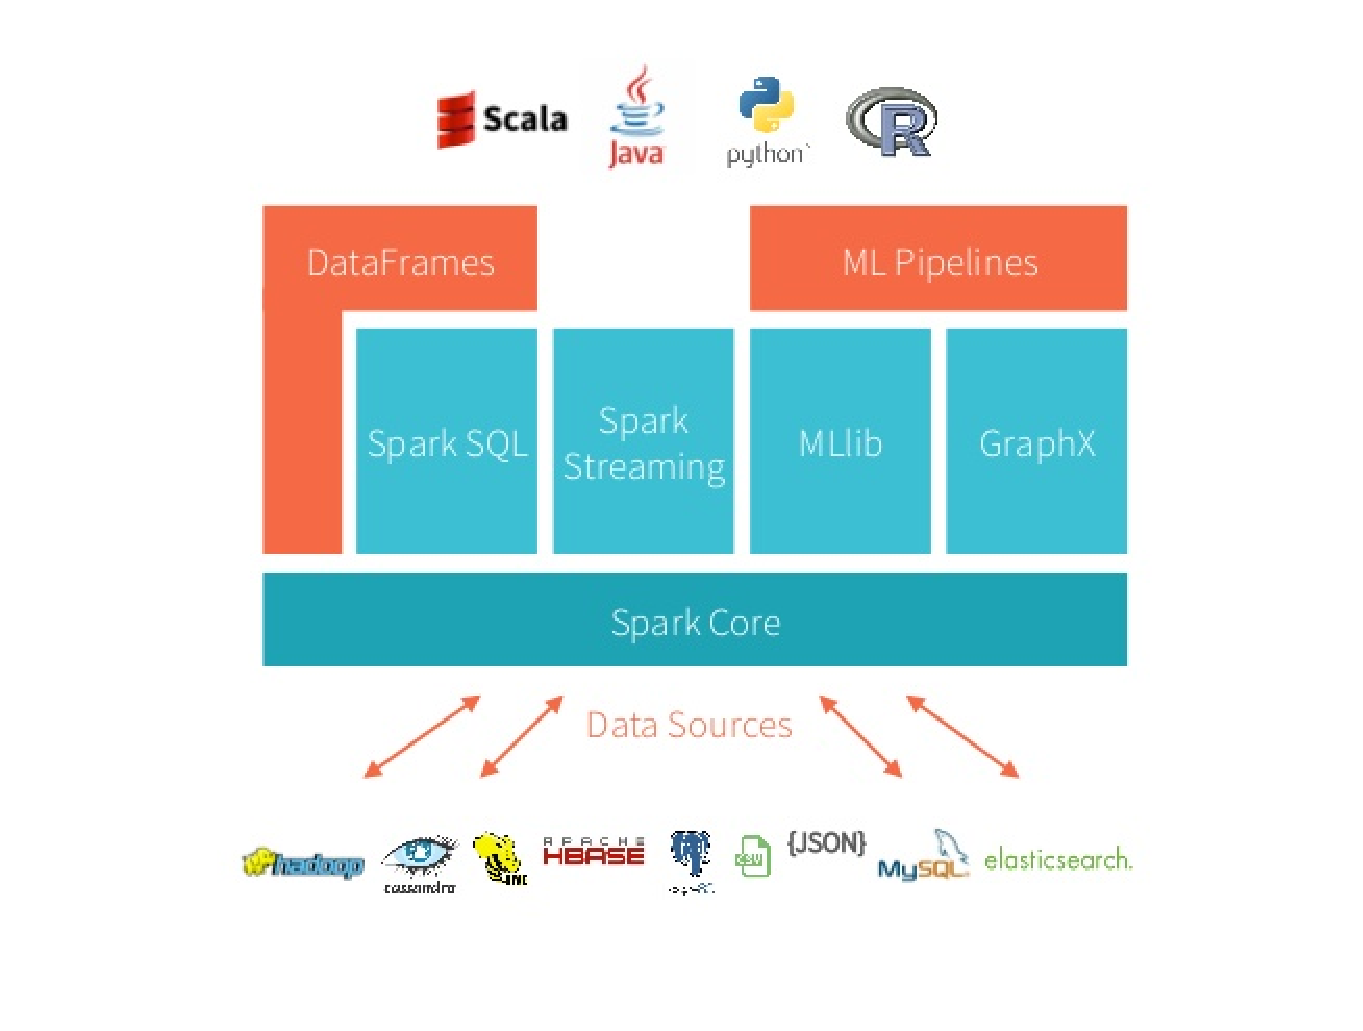
\includegraphics[width=1.0\linewidth]{spark-core}
  \caption{Spark 生态圈}
  \footnotesize 注:图像来源\protect\footnotemark
\end{figure}
\footnotetext{http://www.slideshare.net/rxin/stanford-cs347-guest-lecture-apache-spark?utm\_source=tuicool}
在 Spark 的生态圈中,Spark 的数据来源可以不仅可以从本地系统或者 HDFS 上各种格式的数据,还可以从 HBase、Cassandra 等数据库中的数据。基于在 Spark 的内核,还提供了诸如 Spark Streaming、Spark SQL、MLlib、GraphX 等数据处理的库。开发者可以使用 Scala、Java、Python 甚至是 R 语言编写 Spark 应用程序完成数据处理的任务。
\subsection{弹性分布式数据集}
弹性分布式数据集(Resilient Distributed Datasets,下文简称 RDD)\cite{Zaharia2012}是 Spark 中的分布式内存的抽象。相比于 Hadoop 中的计算过程,RDD 可以被缓存在内存当中,每一次的计算产生的结果都可以保留在内存当中。对于迭代计算,这样多次迭代的计算每次可以将结果保存在内存中,下一次迭代又可以直接从内存中读取数据计算,从而避免了大量的磁盘读写操作,大大节省了计算时间。

一般来说,RDD 的创建是通过 SparkContext 来实现,主要包含有两种创建来源:一是从支持的文件系统(或支持的数据库)读取创建;二是从内存数据集合生成。不同于 Hadoop 中仅有 Map 和 Reduce 操作,RDD 还支持其他类型的操作,主要分为转换操作、控制操作和行为操作三类。转换操作顾名思义,就是将一个 RDD 操作之后转换为另一个 RDD,包括 map、flatMap、filter 等操作。控制操作主要用来将 RDD 缓存到内存中或者磁盘上,比如 cache、persist、checkpoint等操作。行为操作主要分为两类:一类是变成集合或标量的操作,另一类是将 RDD 外部文件系统或数据库的操作。Spark 中的所有对 RDD 的操作,只有当执行行为操作时,才会执行之前的转换或控制操作。例如,我们先对 RDD 执行 map 操作, 然后执行 reduce 操作, 在 map 操作时,Spark 并不会真正执行,只是记录,只有执行 reduce 操作时才会真正一起计算。这一特性称为惰性计算(lazy computing)。图
\ref{fig:rdd} 是对 RDD 的操作流程示例。
\begin{figure}[H]
  \centering
  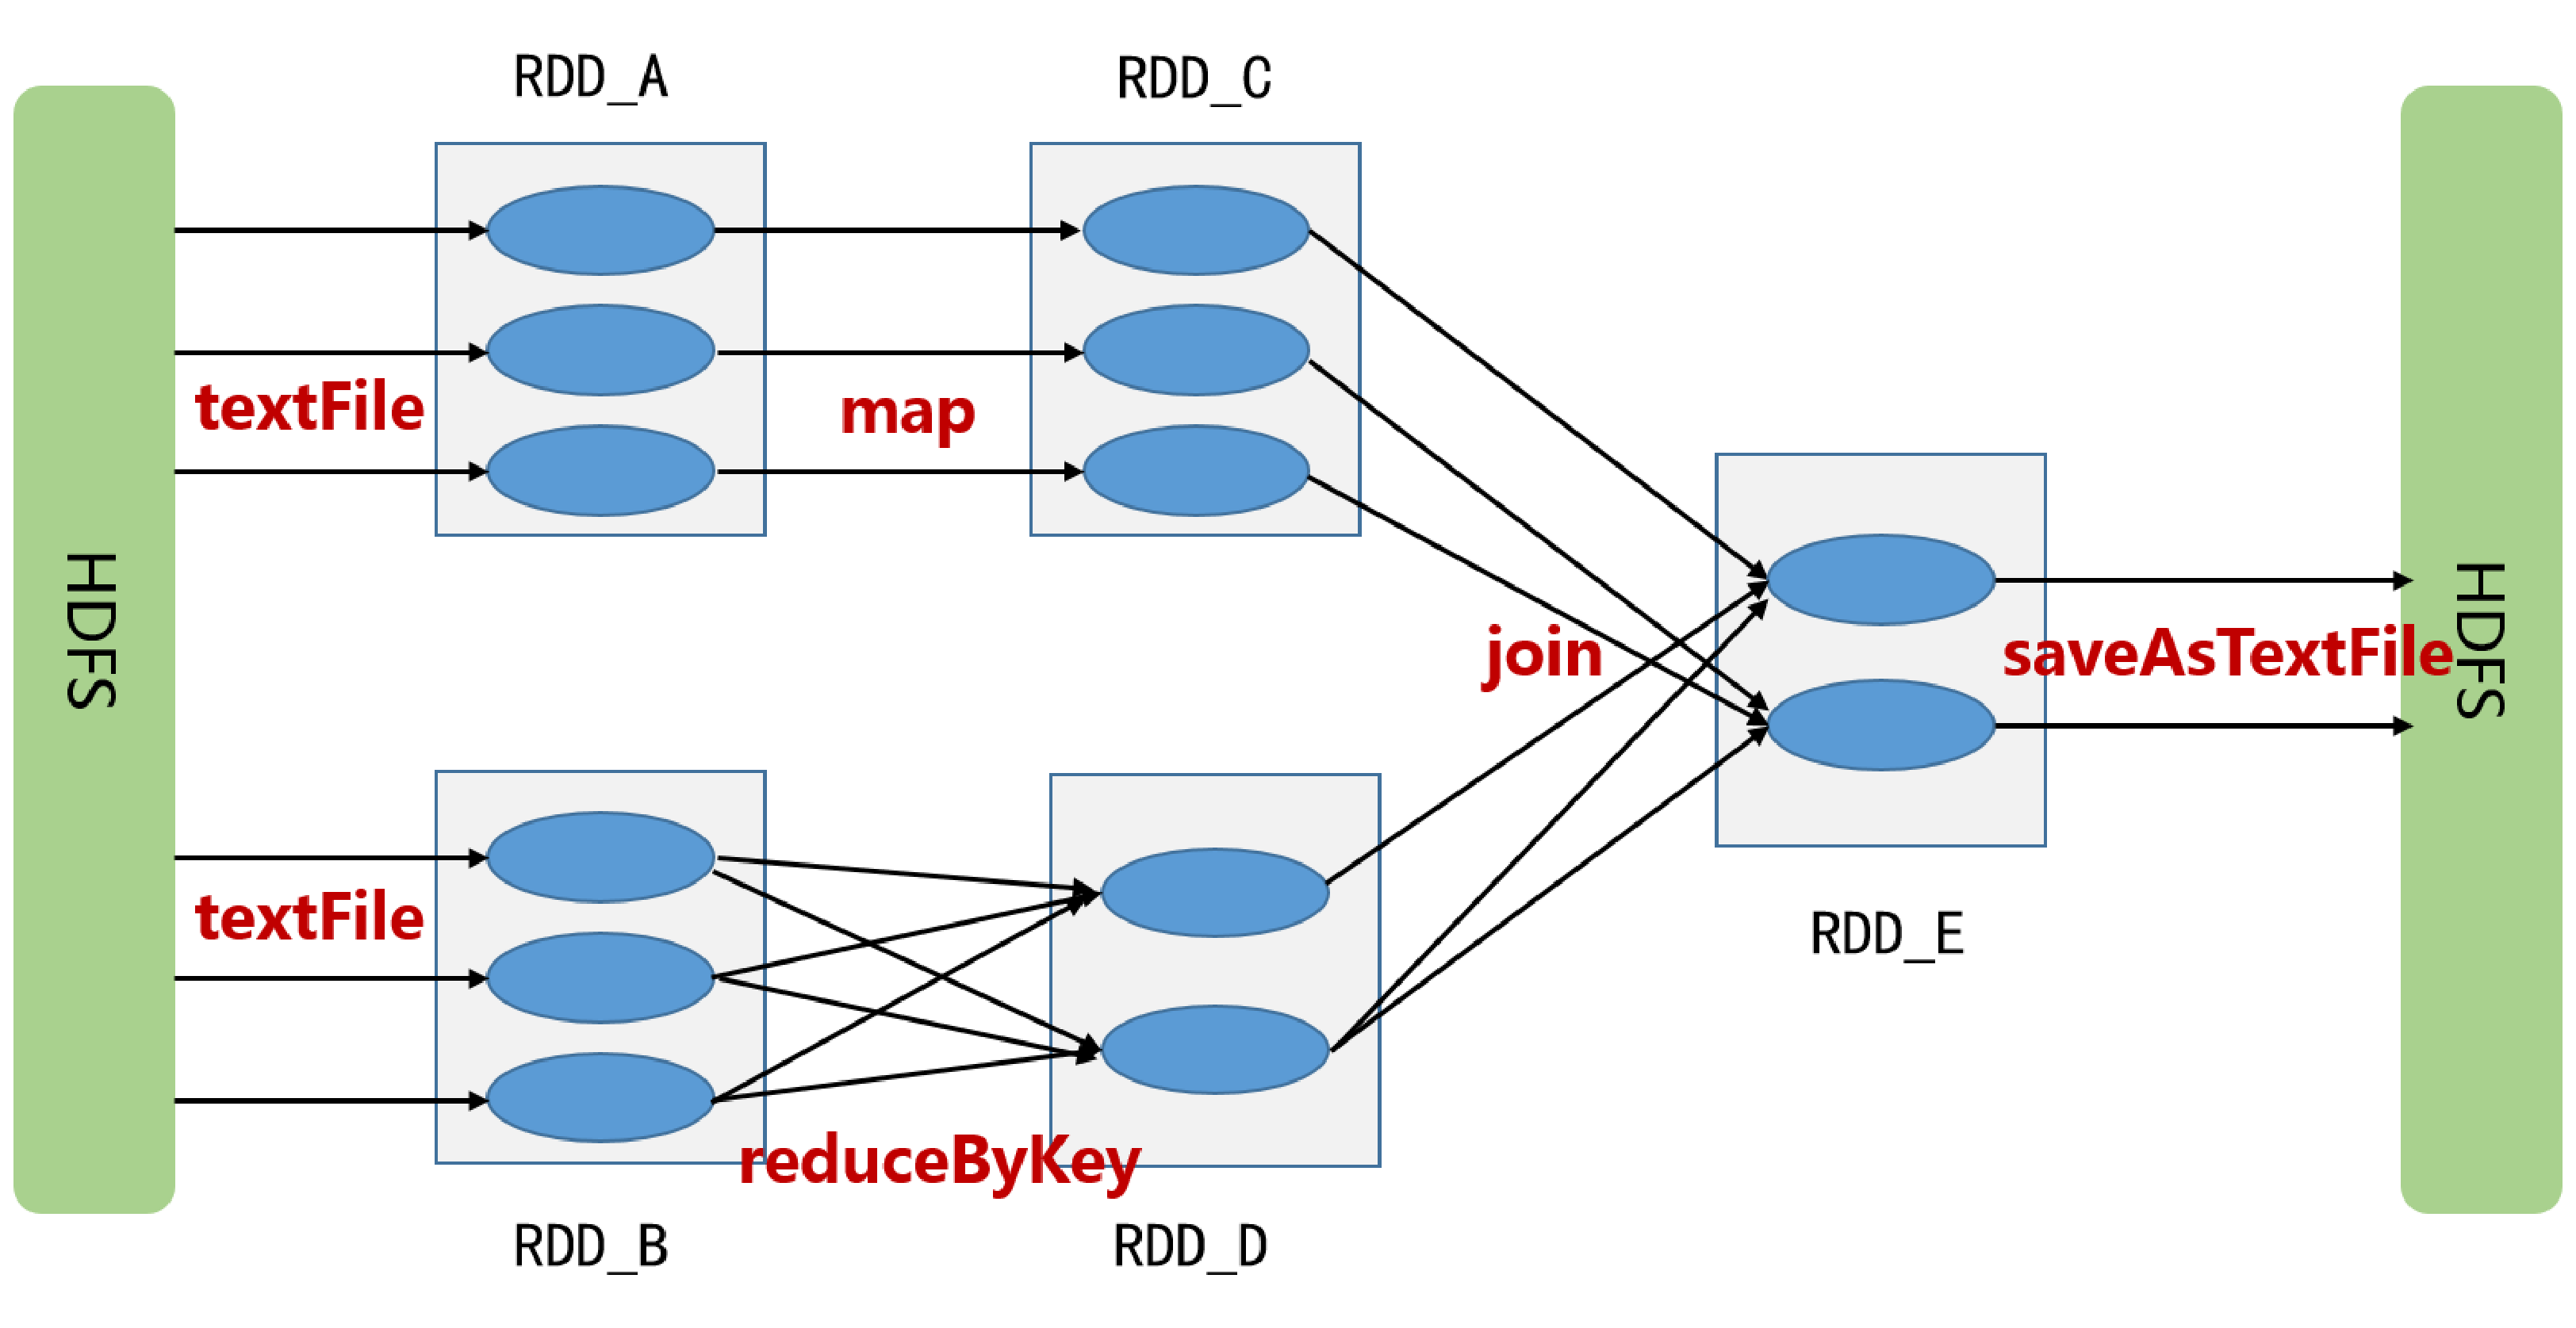
\includegraphics[width=1.0\linewidth]{rdd}
  \caption{RDD 操作流程示例}
  \label{fig:rdd}
\end{figure}

RDD 的持久化是 Spark 中 RDD 的一个重要特性。通过 RDD 的持久化,我们可以将 RDD 缓存到内存或者磁盘上。默认地,RDD 并不会进行缓存,每次计算需要用到 RDD 时,都需要重新计算获取 RDD,这样是非常低效的,特别是对于一些迭代的计算。因此,我们需要考虑在计算过程中,将一些重复用到的 RDD 进行缓存操作,这样我们我们只要第一次计算出 RDD,以后每次用到相同的 RDD 时就不用在重复计算,从缓存中直接读取就可以了。RDD 的 cache() 和 persist() 函数就是用于缓存的,其中 cache() 函数是指将 RDD 缓存在内存当中,而 persist() 根据参数可以将 RDD 进行不同级别的缓存。

RDD 本身自带有容错机制,通过记录 RDD 的演变过程以便在任务执行失败的时候能够恢复出原有的数据,而不需要通过备份的形式实现容错。例如,当前的 RDD 的因任务执行失败而数据丢失,系统则会根据记录的 RDD 演变关系回溯到未丢失的祖先 RDD,重新根据转换操作计算出一个新的 RDD 进行恢复。
\subsection{分布式机器学习库 MLlib}
随着数据量的不断增大,传统的单机式的机器学习算法实现已经无法满足大数据的要求,分布式机器学习算法为解决大数据机器学习的提供了可能。MLlib 是基于 Spark 构建的一个常用分布式机器学习算法和工具库,目前支持的算法包括分类算法、回归算法、聚类算法、协同过滤算法、降维算法等。MLlib 中的分布式机器学习算法,相比于以往的算法,在时间效率有了明显提升。下图(\ref{fig:logistic-regression})是逻辑回归算法在 Hadoop 和 Spark 上的执行时间对比。
\begin{figure}[H]
  \centering
  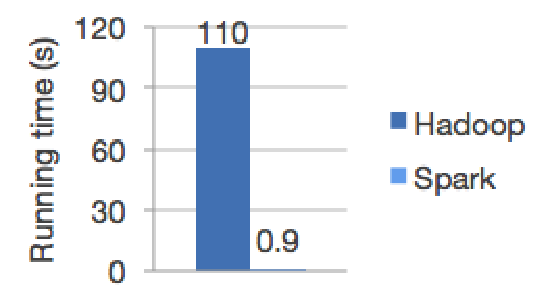
\includegraphics[width=0.3\linewidth]{logistic-regression}
  \caption{Hadoop 和 Spark 上逻辑回归算法效率对比}
  \label{fig:logistic-regression}
  \footnotesize 注:图像来源\protect\footnotemark
\end{figure}
\footnotetext{http://spark.apache.org/}
MLlib 中已经实现的一些常用机器学习算法可以供使用者调用,在 Spark 上利用 MLlib 实现分布式地实现大规模数据的机器学习的任务正是一个不错的选择。
\section{乘积量化}
\label{sec:product_quantization}
与之前提到的 K-Means 的量化方法一样,乘积量化(Product Quantization)\cite{Herve_PQ}也是向量量化方法的一种。假设我们需要量化压缩 128 维的向量到 64 比特,采用 K-Means 的量化方法的话,需要有 $2^{64}$ 个聚类中心,这样不管是从 K-Means 聚类所需要的时间还是从存储聚类中心所占的空间来看,都是不可行的。

对于上面同样的问题,在乘积量化的算法中,我们首先将原始的数据空间划分为 $m$ 个不相交的子空间,也就是将 128 维的向量切成 $m$ 个长度为 $128/m$ 的子向量。在每个子空间里,分别对子空间中的子向量集合进行 K-Means 聚类,聚类中心数量为 $h$。这样我们就可以用 $1\cdots h$ 这些编号来对子向量进行编码,$m$ 个子向量的编码组合在一起就构成了原始向量的编码。这样,原始空间中一个 128 维的向量就可以压缩到一个 $m\log_2h$ 比特编码表示,从而大大节省了空间。
\begin{figure}[H]
  \centering
  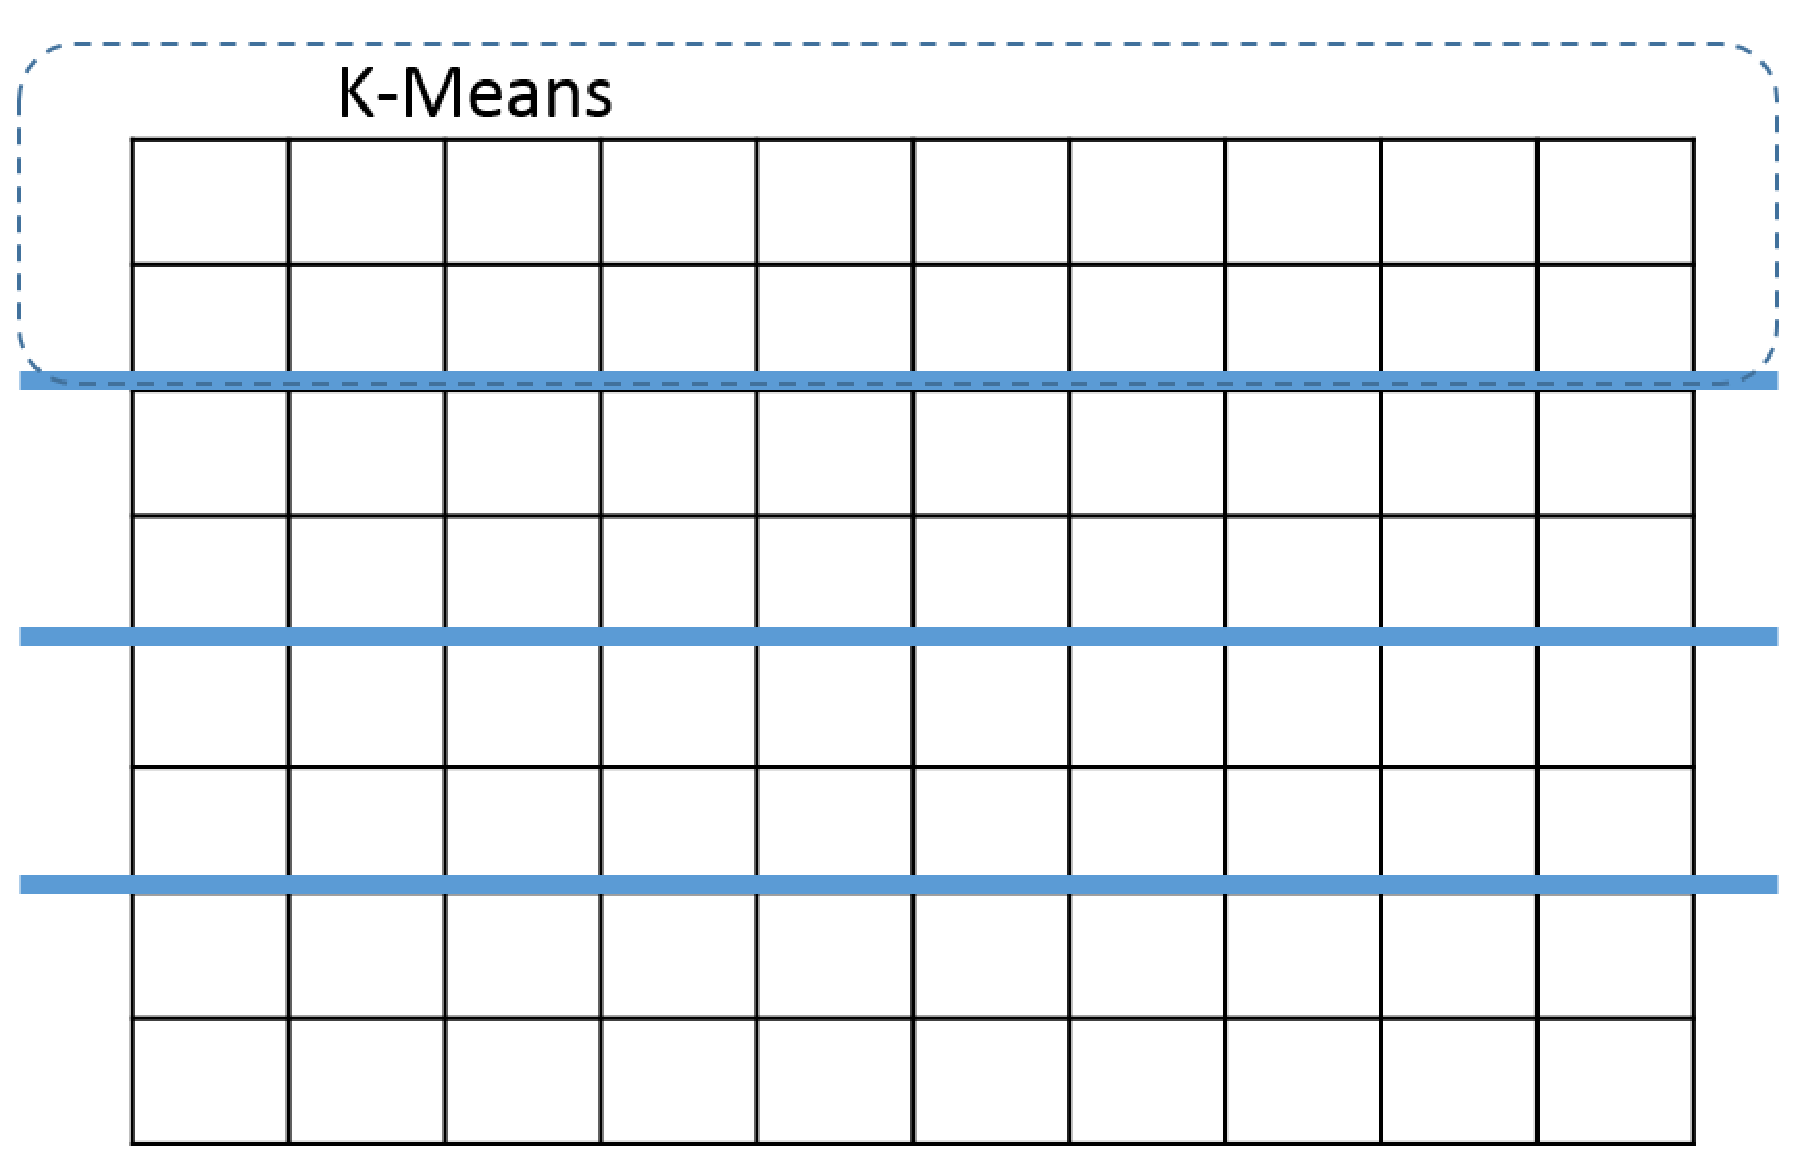
\includegraphics[width=0.5\linewidth]{PQ_subspace}
  \caption{PQ 算法中子空间的划分}
  \label{fig:PQ_subspace}
\end{figure}
更为一般来说,我们可以得到乘积量化方法的目标函数如下:
\begin{equation}
\mathit{l}_\mathrm{PQ} = \sum_{i=1}^n\min\Bigg\lVert \mathbf{x}_i - \begin{bmatrix}C^1\mathbf{b}^1_i\\\vdots\\C^m\mathbf{b}^m_i\end{bmatrix} \Bigg\rVert _2^2
\end{equation}

其中 $\mathbf{x}_i$ 的维度是 $p$,$\mathbf{b}^j_i \in \{0,1\}^h$且$\lVert\mathbf{b}^j_i\rVert=1$,$j \in \{1,\cdots,m\}$。在上面式子中,$C^j(j\in \{1,\cdots,m\})$ 就是我们需要求解的矩阵。在编码过程中,整体的码本(codebook)$C$ 就可以用笛卡尔积的形式表示,$C = C^1 \times \ldots \times C^m$。码本的大小就是所有子空间中聚类中心数量的乘积,根据前面的假设,共有 $m$ 个子空间,每个子空间聚类个数为 $h$,所以码本数量就是 $k = h^m$。求解过程其实并不复杂,正如前文提到,在每个子空间中做 K-Means 聚类就可以求解出码本,这样我们就可以利用码本对每个子空间中的子向量进行编码,从而对原始向量进行编码表示。整个算法的复杂度就和向量维度 $p$、子空间数量 $m$、子空间聚类中心数量 $h$ 有关,存储码本所需要的空间复杂度为 $O(mhp)$。
\begin{table}[htbp]
  \centering
  \caption{乘积量化与 K-Means 量化的空间占用对比}
  \label{tab:kmean_pq}
  \begin{minipage}[t]{0.61\textwidth}
    \begin{tabular}{|c|c|c|c|}
      \hline
                    & 聚类中心 & 编码长度& 空间占用\\
      \hline
      K-Means 量化  &  $k$ &   $\log k$&   $O(kp)$\\
      乘积量化      &   $h^m$ &   $m\log h$ &  $O(mhp)$\\
      \hline
    \end{tabular}\\[2pt]
    \footnotesize 注:$h^m = k$
  \end{minipage}
\end{table}

从表 \ref{tab:kmean_pq} 是乘积量化算法和 K-Means 量化算法的空间占用对可知,当 $m = 1$ 时,乘积量化就退化成普通的 K-Means 聚类量化了。此外, $h$ 取值越大,不仅计算时间复杂度越大,而且空间复杂度也越大,进而也会使得在查询时的时间复杂度变大。因此,选择一个合适的 $m$ 和 $h$ 是非常重要的。论文\cite{Herve_PQ}中指出,$ m = 8 $ 和 $h = 256$ 是比较合适的选择。
\section{基于乘积量化的近似近邻查询}
刚刚我们已经介绍了乘积量化的编码压缩方法,那么如何将这一方法运用在近似近邻查询当中呢?采用乘积量化的方法进行近似近邻查询也是一个机器学习类方法,遵循学习类算法的主体流程。整个近似近邻查询算法的主要流程如下:
\begin{itemize}
\item 利用部分数据集,依照乘积量化的方法训练出码本。
\item 在原始的数据集上,采用训练出的码本对其进行编码压缩。
\item 对于任意的查询向量,度量它与编码压缩后的码字之间的距离,从而得到近邻集合。
\end{itemize}
\subsection{训练码本}
首先是训练集的选择,训练集的选取对整个算法是非常关键的,最终近邻查询的准确率一定程度上取决于训练集的好坏。在选择训练集上有两点需要注意,一是训练集的规模大小,二是训练集的代表性。训练集的规模既不宜过大也不能太小,过大会带来过拟合问题,过小则会欠拟合。通常,训练集的规模大小约为原始数据集的 $1/10$ 比较合适。此外,训练集还应该尽可能得有代表性,尽可能广泛地分布于整个数据空间,这样才能使得训练出来的码本才能更好的量化原始数据空间,更准确地对原始数据集进行编码。

在具体训练码本的过程中,如章节 \ref{sec:product_quantization} 中所介绍的一样,首先将训练集中的数据划分到 $m$ 个子空间。在每个子空间中,对所有的子向量数据在进行 K-Means 聚类,可以得到 $h$ 个聚类中心,也就得到每个子空间的码本。算法的伪代码如算法 \ref{algo:train} 所示。
\begin{algorithm}
    \caption{训练码本}
    \label{algo:train}
    \begin{algorithmic}[1] %每行显示行号
        \Require 训练集 $C$ 矩阵,子空间聚类数量 $subCenters$,聚类算法最大迭代次数 $maxIterations$
        \Ensure 码本模型数组 $model$
        \Function {PQ\_TRAIN}{$C, subCenters, maxIterations$}
            \State uniformly split $C$ by rows into $m$ part
            \For{$i = 1 \to m $}
                \State $model[i] \gets KMEANS\_TRAIN(C[i], subCenters, maxIterations)$
            \EndFor
            \State \Return{$model$}
        \EndFunction
    \end{algorithmic}
\end{algorithm}
\subsection{编码压缩}
如算法 \ref{algo:assgin} 所示,训练得出每个子空间中的码本之后,将其应用到原始数据集上进行编码压缩。首先,同样也是将原始数据集划分到 $m$ 个子空间。然后在每个子空间中,对每一个数据的子向量,分别用训练出来的码本进行编码,也就是用训练好的 K-Means 模型进行预测,可以知道每个子向量隶属于哪个聚类中心,即子向量应该用哪个码字来编码了。这样,整个数据集中的数据都可以用编码来进行表示。完成编码压缩之后,编码后的数据集相比于原始数据集,存储空间成倍的缩小了。
\begin{algorithm}
    \caption{编码压缩}
    \label{algo:assgin}
    \begin{algorithmic}[1] %每行显示行号
        \Require 码本模型数组 $model$,原始数据集 $X$ 矩阵
        \Ensure 编码后的矩阵 $B$
        \Function {PQ\_ASSIGN}{$model, X$}
            \State uniformly split $X$ by rows into $m$ part
            \For{$i = 1 \to m $}
                \For{$j = 1 \to n $}
                    \State $B[i][j] \gets model[i].predict(X[i][j])$
                \EndFor
            \EndFor
            \State \Return{$B$}
        \EndFunction
    \end{algorithmic}
\end{algorithm}
\subsection{近邻查询}
在近似近邻查询的过程中,对于任意一个查询向量 $q$,我们首先计算出 $q$ 在子空间中对应子向量和子空间中聚类中心之间的距离,将计算出的距离用一个查找表存储好。现在我们计算查询向量 $q$ 和编码数据集上的每个数据之间的距离。在每个子空间中,因为我们已经计算出了子向量与聚类中心之间距离,利用查找表,我们就可以迅速得出每个数据在子空间中与向量对应距离。最终将不同子空间中同一向量距离加和。这样就得到了最终的每个向量和查询向量 $q$ 之间的距离。利用一个优先队列,我们就可以快速获取出前 $k$ 个近邻集合。具体算法流程可以参考算法 \ref{algo:ANNS}
\begin{algorithm}
    \caption{近邻近邻查询}
    \label{algo:ANNS}
    \begin{algorithmic}[1] %每行显示行号
        \Require 码本模型数组 $model$,编码数据集 $B$ 矩阵,查询数据 $q$
        \Ensure 近邻集合 $result$ 数组
        \Function {PQ\_SEARCH}{$model, B, q$}
            \For{$i = 1 \to m $}
                \For{$j = 1 \to model[i].subcenters $}
                    \State $d[i][j] \gets COMPUTE\_DIST(model[i].center[j], q) $
                \EndFor
            \EndFor

            \For{$i = 1 \to n $}
                \State $dist[i] \gets 0$
                \For{$j = 1 \to m $}
                    \State $dist[i] \gets dist[i] + d[i][B[j][i]]$
                \EndFor
            \EndFor
            \State $result = GET\_TOPK(dist)$
            \State \Return{$result$}
        \EndFunction
    \end{algorithmic}
\end{algorithm}
\section{基于 Spark 的分布式近似近邻查询}
\subsection{算法流程设计}
算法的总体流程设计图如图 \ref{fig:algorithm-desgin} 所示,首先在训练数据集上进行码本的训练,得到码本模型后将其运用在原始数据集上进行编码压缩,从而可以将原始数据进行编码表示。最终,对于任意一个查询向量,通过近似近邻查询算法在编码数据集上找出近邻候选集合。
\begin{figure}[H]
  \centering
  \includegraphics[width=0.8\linewidth]{algorithm-desgin}
  \caption{算法总体设计图}
  \label{fig:algorithm-desgin}
\end{figure}
\subsection{数据结构}
在 Spark 上,分布式程序的编写必须依赖分布式的数据结构 RDD, RDD 分布式地存储在不同节点上,这样才能保证程序分布式地执行 。因此如何合理设计程序的 RDD 非常重要。

在 Spark MLlib 库中提供了一种自带的数据结构 BlockMatrix。BlockMatrix 是用 RDD 构建的分布式矩阵,其中 RDD 的类型是 ((Int, Int), Matrix)。(Int,Int)是 Matrix 的下标索引,那么 BlockMatrix 的每一个元素都是一个带下标索引的矩阵。BlockMatrix 还提供了一些自带的函数可供调用,如 add、multiply。

\begin{figure}[H]
  \centering
  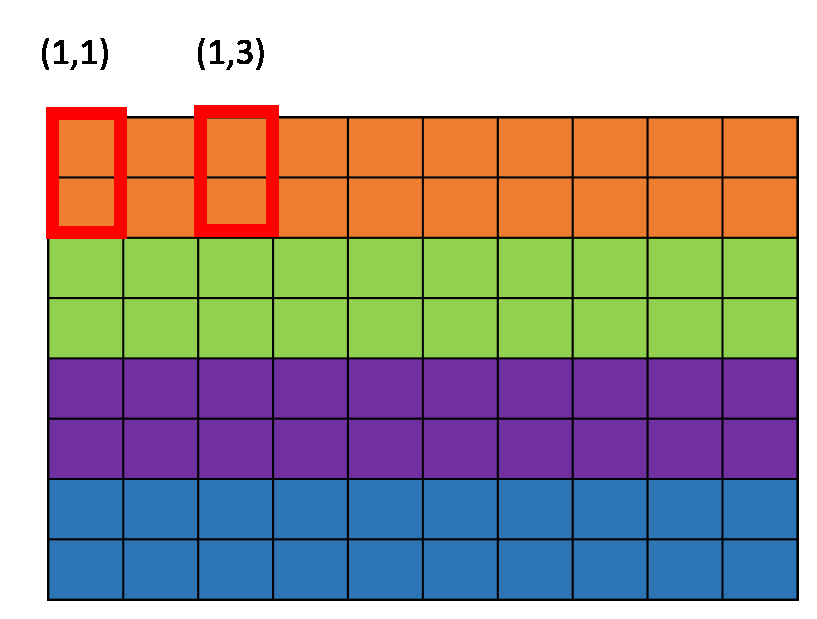
\includegraphics[width=0.6\linewidth]{blockmatrix}
  \caption{BlockMatrix 划分方式}
  \label{fig:blockmatrix}
\end{figure}

图 \ref{fig:blockmatrix} 是一个示例的 BlockMatrix 的划分方式,图中的$ 8\times 10$ 的矩阵被划分成 4 个子空间,每个子空间上有 10 个子向量。那么我们需要一个 $4\times 10$ 的 BlockMatrix 来存储,红色的框中的向量就对应了一个 matrix,相应 matrix 的下标索引标示在图中了。在上一章节的算法中已经说明,我们需要划分 $m$ 个子空间,每个子空间中有 $n$ 个子向量,因此我们用 $m\times n$ 的 BlockMatrix 数据结构来表示数据是比较合适的。具体而言,我们算法中的训练集数据、原始数据、编码后的数据等都是需要用 BlockMatrix 这个数据结构来存储表示的。
\subsection{系统优化}
集群系统上的分布式程序一般来说都会需要考虑通信的问题,即使 Spark 中 RDD 已经进行了很好的封装,让开发者可以不用直接进行底层的数据管理(通信、容错),只需要通过操作上层的一些 API 就可以了,但是数据通信的问题在 Spark 中还是一个不能忽视的,只有了解底层的通信机制才能利用 API 编写出高效的程序。一般来说,我们优化的原则是尽可能地减少数据的通信,特别是通信量比较大的数据通信。

数据都是分布式存储,如果某个操作与两个分布式数据同时关联,比如两个大小相同分布式矩阵对应元素相加,那么必须要两个分布式数据中分块的一一对齐。具体到本算法中,根据上一小节所提的数据结构的划分方式,假设存储训练数据集的矩阵用 $C$ 表示,存储原始数据集 BlockMatrix 用 $X$ 表示,存储编码后数据集的矩阵用 $B$ 表示,这些都是分布式地存储在集群系统当中的。由于子空间的划分,我们会在每个子空间中生成自己的码本模型。如果码本模型是分布式存储,那么在编码阶段,我们需要将子空间对齐。 Spark RDD 的 join 操作确实提供了按照键值进行对齐操作,但这一过程可能就会产生一些数据分区重组操作。这种分区重组的操作需要进行磁盘读写和网络通信,因此我们应该尽量避免分区重组操作。我们考虑采用 RDD 的广播操作,一次性将只读的数据广播到集群上的所有节点,每个节点上的任务在执行过程中可以直接读取,而不需要考虑对齐问题。在我们算法中,我们选择将计算出的码本模型广播到所有节点以便编码阶段使用。

第二点优化就是利用之前提到的 Spark RDD 的持久化机制。Spark RDD 的持久化可以将 RDD 数据缓存到内存或者磁盘上,以后用到 RDD 的时候不要再次重复计算,从而节省时间效率,这一机制特别适合迭代计算中使用。在我们的算法中,我们选择将一些反复用到 RDD 缓存在内存当中。
\section{本章小结}
本章中首先介绍了 Spark 的弹性分布式数据集合分布式机器学习库 MLlib,接着介绍了乘积量化的哈希方法,通过乘积量化的方法将原始数据集进行编码压缩。之后,我们还介绍了乘积量化哈希方法在近似近邻查询中应用。通过训练码本、编码压缩、近似近邻查询三个过程,我们就可以实现一套完整的近似近邻查询算法。此外,本章节还介绍了在 Spark 计算框架上的这一算法的实现,主要介绍了算法总体流程设计、数据结构的选择以及系统的优化方法。




%%% Local Variables:
%%% mode: latex
%%% TeX-master: t
%%% End:

\chapter{基于 Spark 的分布式近似近邻查询系统}
\label{cha:ANNS_based_on_Spark}
\section{乘积量化}
与之前提到的 K-Means 的量化方法,乘积量化(Product Quantization)\cite{Herve_PQ}也是向量量化的一种。假设我们需要量化压缩 128 维的向量到 64 比特,采用 K-Means 的量化方法的话,需要有 $2^{64}$ 个聚类中心,这样不管是从 K-Means 聚类所需要的时间还是从存储聚类中心所占的空间来看,都是不可行的。

对于上面同样的问题,在乘积量化的算法中,我们首先将原始的数据空间划分为 $m$ 个不相交的子空间,也就是将 128 维的向量切成 $m$ 个长度为 $\frac{128}{m}$ 的子向量。在每个子空间里,分别对子空间中的子向量集合进行 K-Means 聚类,聚类中心数量为 $h$。这样我们就可以用 $1\cdots h$ 这些编号来对子向量进行编码,$m$ 个子向量的编码组合在一起就构成了原始向量的编码。这样,原始空间中一个 128 维的向量就可以压缩到一个 $m\log_2h$ 比特编码表示,从而大大节省了空间。
\begin{figure}[H]
  \centering
  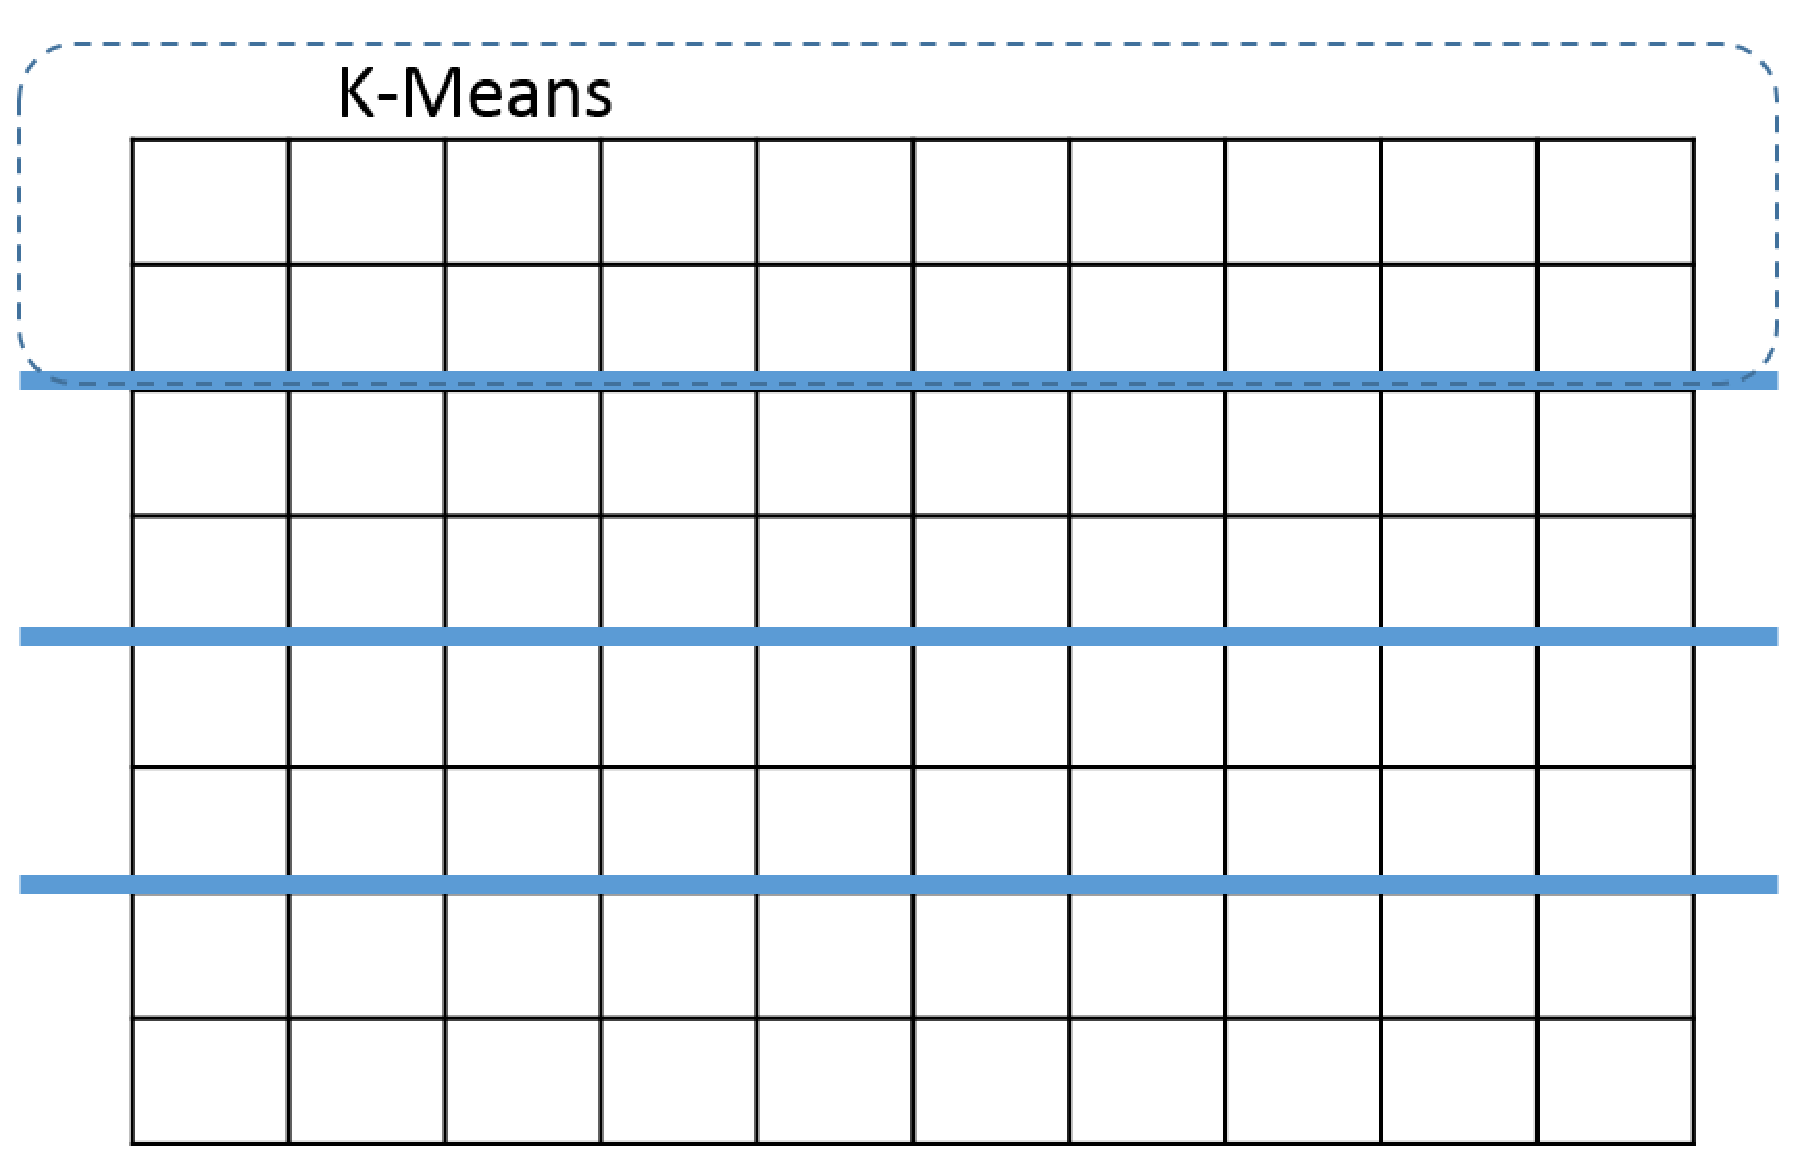
\includegraphics[width=0.5\linewidth]{PQ_subspace}
  \caption{PQ 算法中子空间的划分}
  \label{fig:PQ_subspace}
\end{figure}
更为一般来说,我们可以得到乘积量化方法的目标函数如下:
\begin{equation}
\mathit{l}_\mathrm{PQ} = \sum_{i=1}^n\min\Bigg\lVert \mathbf{x}_i - \begin{bmatrix}C^1\mathbf{b}^1_i\\\vdots\\C^m\mathbf{b}^m_i\end{bmatrix} \Bigg\rVert _2^2
\end{equation}
其中 $\mathbf{b}^j_i \in \{0,1\}^h$且$\lVert\mathbf{b}^j_i\rVert=1$,$j \in \{1,\cdots,m\}$。在上面式子中,$C^j(j\in \{1,\cdots,m\})$ 就是我们需要求解的矩阵,在编码过程中,我们称其作为码本(codebook)。求解过程其实并不复杂,正如前文提到,在每个子空间中做 K-Means 聚类就可以求解出码本,这样我们就可以利用码本对每个子空间中的子向量进行编码,从而对原始向量进行编码表示。
\section{利用乘积量化的近似近邻查询}
前文所提的乘积量化只是介绍了如何进行数据的压缩编码,那么乘积量化到底如何应用到近似近邻查询当中呢?
\section{Spark 上的分布式实现}
\subsection{RDD 的划分}
\subsection{训练阶段}
\subsection{编码阶段}
\subsection{查询阶段}



%%% Local Variables:
%%% mode: latex
%%% TeX-master: t
%%% End:

\chapter{实验与分析}
\label{cha:experiments_analysis}
本章节主要介绍在 Spark 集群上进行近似近邻查询算法的实验,主要包括实验环境介绍、实验数据集介绍、实验结果展示以及实验分析。
\section{实验环境}
本次实验中关于 Spark 部分的实验都是在由 4 台机器构成的 Spark on YARN 集群系统上完成的。其中,每台机器配置均相同,配置如下:
\begin{itemize}
\item 操作系统:Red Hat Enterprise Linux Server release 7.0
\item 处理器信息:Intel(R) Xeon(R) CPU E5-2609 0 @ 2.40GHz
\item 核数:8 核
\item 内存大小: 60G
\end{itemize}

关于 MATLAB 部分的实验是在一台单机上完成,配置如下:
\begin{itemize}
\item 操作系统:Windows 8
\item 处理器信息:Intel(R) Core(TM) i3 CPU M 380 @ 2.53GHz
\item 核数:4 核
\item 内存大小: 6G
\end{itemize}
\section{实验数据集}
实验过程中主要使用到了两个数据集,一个是 SIFT1M\footnote{http://corpus-texmex.irisa.fr/},另一个是 CIFAR-10\footnote{http://www.cs.toronto.edu/~kriz/cifar.html}。实验主要对比笔者实现的方法在 Spark 集群系统上与 MATLAB 单机系统上的近似近邻查询的召回率以及相应时间消耗,此外也对比在不同的参数下, Spark 集群系统上的运行结果。
\subsection{SIFT1M}
SIFT1M 是近年来被广泛应用于近似近邻查询方法准确率和召回率的衡量。这个数据集中的数据都是 128 维的 SIFT 特征向量,包含三部分:待索引的原始数据集(base)、训练数据集(learn)、查询数据集(query)。其中待索引的原始数据集合有 $10^6$ 个向量,训练数据集有 $10^5$ 个,查询数据集共有 $10^4$ 个。
\subsection{CIFAR-10}
CIFAR-10 数据集被广泛用于在计算机视觉领域做目标识别、图像分类等任务的。它是从 80 million tiny images\footnote{http://groups.csail.mit.edu/vision/TinyImages/} 数据集中挑选出的一个带标签的子集,由 60000 张 $32\times 32$ 的彩色图像组成。它们被分成 10 类,每个类别有 6000 张图片。10 个类别分别是airplane、automobile、bird、cat、deer、dog、frog、horse、ship、truck。

\begin{figure}[H]
  \centering
  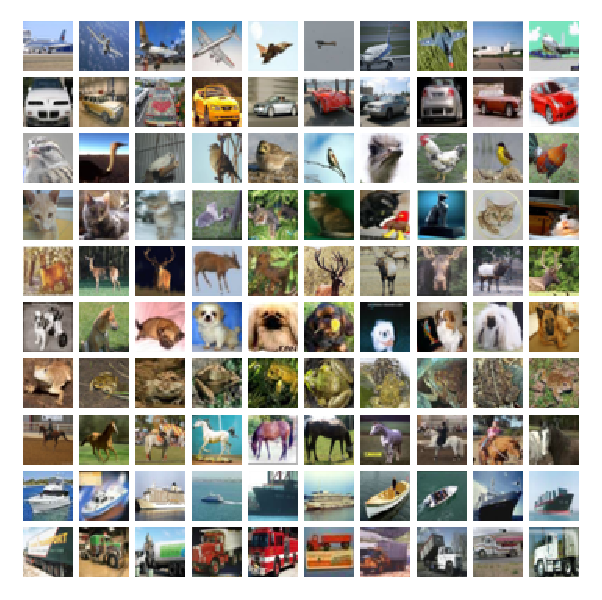
\includegraphics[width=0.7\linewidth]{cifar-10}
  \caption{CIFAR-10 数据集中图片示例}
  \label{fig:cifar-10}
\end{figure}
\section{实验结果与分析}
\subsection{Spark 集群与 MATLAB 对比实验}
本实验室在 SIFT1M 数据上进行,通过比较 Spark 集群上的乘积量化的近似近邻查询方法与 同样方法在 MATLAB 单机上的实验的召回率和时间消耗的对比。

在 Spark 集群系统上的程序参数设置,我们采用 yarn-client 模式在集群上运行程序,设置 executor 的数量为 40,每一个 executor 的内存大小限制为 5G。在对 SIFT1M 数据集近似近邻查询实验中,我们设置子空间切分数量 $m$ 为 8,子空间中的聚类中心数量为 $h$ 为 256,因此总的聚类中心的数量就是 $2^64$,编码字节的大小就是 64 比特。$h$ 取 256 是比较合适的,恰当的子空间聚类中心数量一方面可以使得查找表的大小不会过大,另一方面保证训练和编码的时间也不会太长。在这次实验中,我们采用 recall@$R$ 作为查询效果好坏的衡量标准。SIFT1M 数据中有 $10^4$ 个查询向量,对于一个查询向量,通过整个近似近邻查询计算,我们在原始向量中找到前 100 个近邻向量,并分别取 $R$ 为 1、2、5、10、20、50、100,计算前 $R$ 个向量中出现最近邻向量的次数 $s$,那么衡量标准就可以由公式 recall@$R = s/10^4$ 计算得出。
\begin{table}[htbp]
\noindent\begin{minipage}{0.5\textwidth}
\centering
\caption{Spark 与 MATLAB 上召回率对比}
\label{tab:recall_on_spark_matlab}
\begin{tabular}{ccc}
\toprule[1.5pt]
    & Spark & MATLAB\\
  \hline
  recall@1  &  0.23   & 0.29\\
  recall@2  &  0.33 &   0.40\\
  recall@5  &  0.48 &   0.53\\
  recall@10  & 0.60 &   0.62\\
  recall@20  &  0.72&  0.73\\
  recall@50  &  0.85 &  0.81\\
  recall@100  & 0.92 &  0.88\\
\bottomrule[1.5pt]
    \end{tabular}
\end{minipage}
\begin{minipage}{0.5\textwidth}
\centering
\caption{Spark 与 MATLAB 上时间对比}
\label{tab:time_on_spark_matlab}
\begin{tabular}{ccc}
\toprule[1.5pt]
    & Spark & MATLAB \\
\hline
训练时间(s) & 1193.04 & 1574.09  \\
编码时间(s) & 12.42 & 49.93 \\
单次查询时间(s)& 2.8 & 181.73 \\
\bottomrule[1.5pt]
\end{tabular}
\end{minipage}
\end{table}
表 \ref{tab:recall_on_spark_matlab} 和表 \ref{tab:time_on_spark_matlab} 分别显示的是在 Spark 上与 MATLAB 中的召回率对比以及所用时间对比。仅从表 \ref{tab:recall_on_spark_matlab} 来看,Spark 集群系统上程序的召回率与 MATLAB 单机版本的相差不大。在保证召回率差不多的情况下,我们再看表  \ref{tab:time_on_spark_matlab},从表中我们可以看出在训练阶段的时间消耗上,Spark 比 MATLAB 耗时要少,但是并没有成倍数介绍。在编码阶段时间消耗, Spark 集群上用时仅为 MATLAB 的 $1/4$ 左右。到了查询阶段,单次耗时 MATLAB 是 Spark 集群系统上单次耗时的 $70$ 余倍。



%%% 其它部分
\backmatter

\makeatletter
  \listoffigures
  \listoftables
  \listofequations
\makeatother


% 参考文献
\bibliographystyle{thubib}
\bibliography{ref/refs}


% 致谢
%%% Local Variables:
%%% mode: latex
%%% TeX-master: "../main"
%%% End:

\begin{ack}
    感谢我的导师王建民教授,王老师严谨治学、勤恳工作的态度深深影响了我。
    
    感谢龙明盛学长对我毕设的耐心指导。同时,也要感谢研究组里的各位学长和学姐,没有他们的答疑解惑,我的毕设工作不可能顺利完成。
    
    感谢大学四年言传身教的各位老师,他们不仅教给我文化知识,而且也教会我为人处世之道。
    
    感谢软件学院一字班里的每一位同学,四年来我们共同学习、互帮互助、共同成长。
    
    感谢林梓佳辅导员四年来的悉心指导和照顾,在我最困难的时候,给予我鼓励和帮助,谢谢林导!
    
    最后,还要感谢在背后一直默默支持我的家人和朋友,谢谢你们!
\end{ack}


% 附录
\begin{appendix}
%%% Local Variables:
%%% mode: latex
%%% TeX-master: "../main"
%%% End:

\chapter{外文资料的调研阅读报告}
\label{cha:engorg}
As one of the most widely used techniques in operations research, {\em
  mathematical programming} is defined as a means of maximizing a quantity known
as {\em objective function}, subject to a set of constraints represented by
equations and inequalities. Some known subtopics of mathematical programming are
linear programming, nonlinear programming, multiobjective programming, goal
programming, dynamic programming, and multilevel programming$^{[1]}$.

It is impossible to cover in a single chapter every concept of mathematical
programming. This chapter introduces only the basic concepts and techniques of
mathematical programming such that readers gain an understanding of them
throughout the book$^{[2,3]}$.
\end{appendix}

\end{document}
